\section{Performance Evaluation}

In this section, we show that:

\begin{itemize}

\item In the network with fixed bandwidth, compared with state-of-the-art VR streaming system, PQVRS saves 45\% bandwidth on average while providing the same PSPNR, or provides 15-20 higher PSPNR in the same bandwidth.

\item In the network with unstable bandwidth, PQVRS improves 10 higher PSPNR and decreases 50\% stalling.

\item In real-world perceived quality rating by users, PQVRS can obtain better user rating.

\item Improvement analysis shows that PQVRS has substantial improvement on ... video segments, and has marginal improvement on ... video segments.

\end{itemize}

\subsection{Evaluation Setup}

To evaluate the performance, we implement PQVRS, a real-world VR streaming system which adaptively choose the quality of each part of video and display on HMD. Fig. \ref{network} shows the network topology in the experiment, which consists of a client and a server.

\begin{figure}
  \centering
  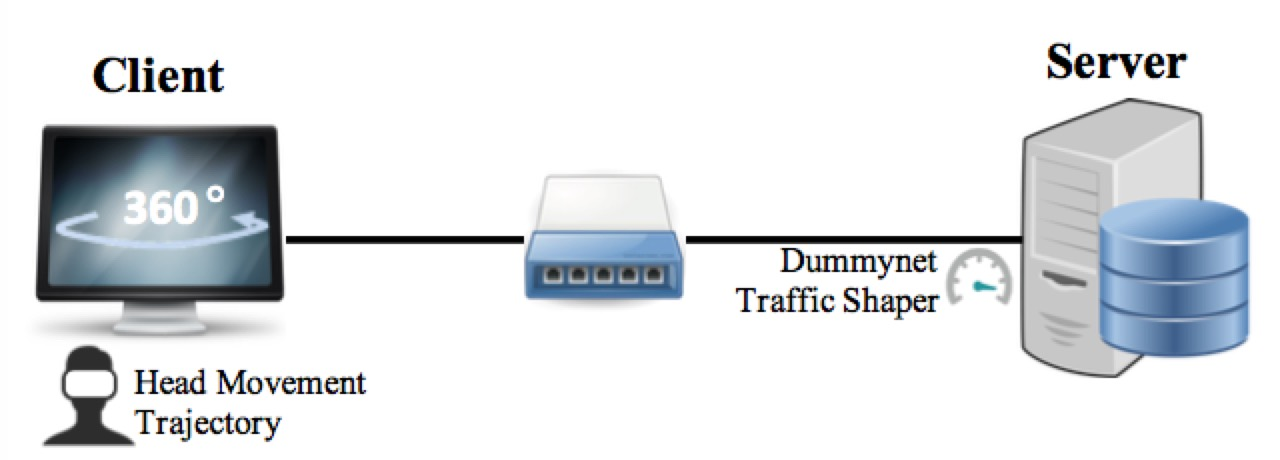
\includegraphics[width=3in]{images/network.jpg}
  \caption{Network topology.}
  \label{network}
  \end{figure}

In the experiments, we choose 50 videos with different types and lengths. We set the duration of one video segment as 1 second. To generate different quality videos, we use quantization parameter (QP) ranging from 22 to 42 in steps of five leading to five different bitrate versions. 

In our experiment, 3 VR streaming systems are chosen to make comparison:

\begin{itemize}

\item \emph{Flare \cite{Flare}:} A state-of-the-art viewpoint-driven VR streaming. Video is cut into 4*6 spatial rectangular tiles. Tiles on user's viewpoint is allocated the high bitrate. For other tiles, bitrate is allocated linearly decreasing with its distance to user's viewpoint.

\item \emph{PQVRS-:} Video is cut into 6*12 spatial rectangular tiles. With consideration of user viewpoint, content luminance and texture complexity, we do adaptive streaming to maximize user-perceived quality.

\item \emph{PQVRS:} Our proposed method in this paper. Object-based video tiling is used to cut video into tiles with different size. Besides user viewpoint, content luminance and texture complexity, we also take consideration of viewpoint moving speed, content Depth-of-Field and light / dark adaptation, and do adaptive streaming to maximize user-perceived quality.

\end{itemize}

\subsection{Performance comparison under fixed bandwidth}

When network is under a fixed bandwidth, video streaming is stalling-free since the requested video segment will always be retrieved back to client on time. User perceived quality is almost only related to PSPNR. So we test the PSPNR-bandwidth tradeoff for above methods under fixed bandwidth. Fig. \ref{practical_imp} shows the result.

  \begin{figure}
  \centering
  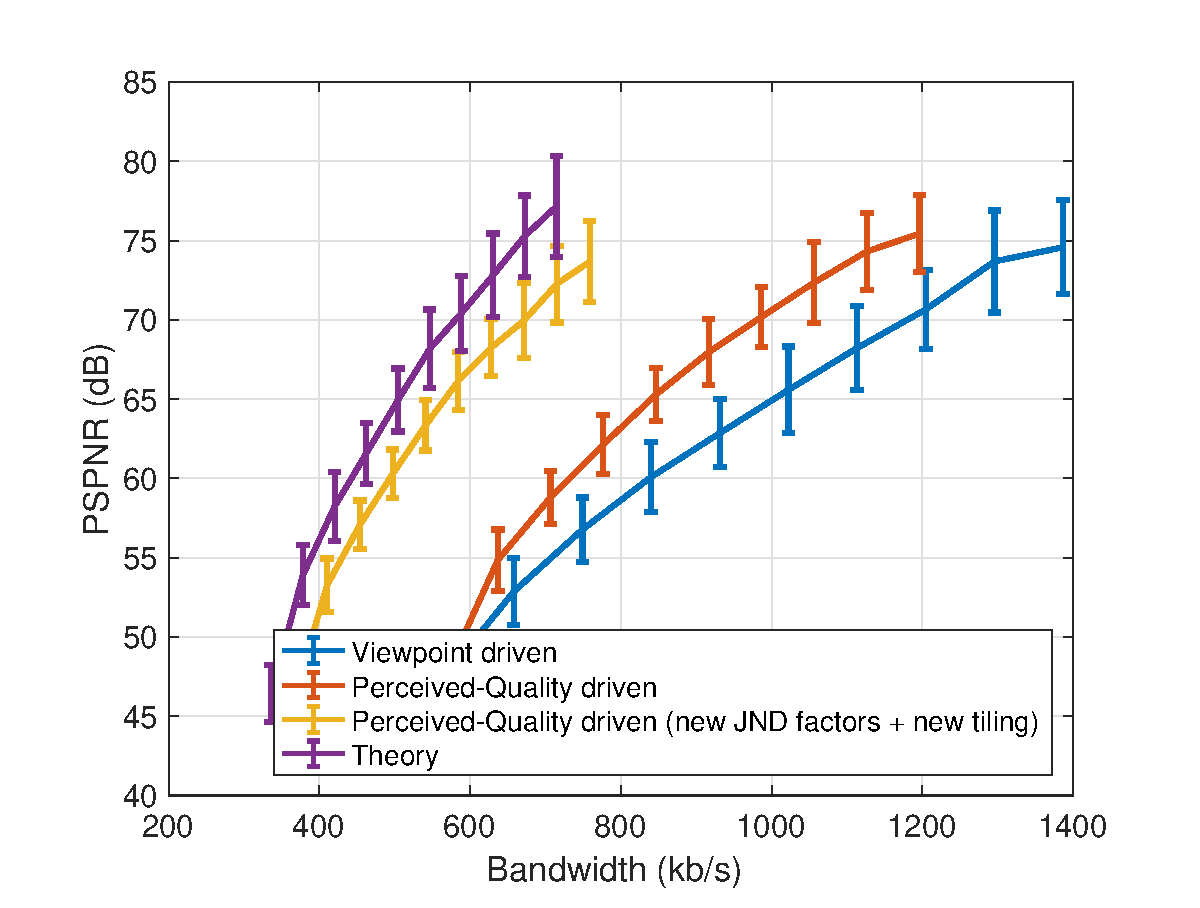
\includegraphics[width=3in]{images/practical_improvement.eps}
  \caption{PSPNR-bandwidth tradeoff of 4 methods: Viewpoint-driven, PQVRS-, PQVRS, theoretical performance.}
  \label{practical_imp}
  \end{figure}

\textbf{Key observations:}

\subsection{Performance comparison under real-world bandwidth}

Actually, in real-world video streaming, bandwidth is unstable which may change significantly in a short time. When the bandwidth change dramatically from a high level to a low level, it not only decrease the value of PSPNR, but also causes stalling in video display, which is another important metric of perceived quality.

We test the performance of Viewpoint-driven, PQVRS-, PQVRS under the network with 800 kb/s bandwidth on average, but with different levels of bandwidth fluctuation. 

   \begin{figure}
  \centering
  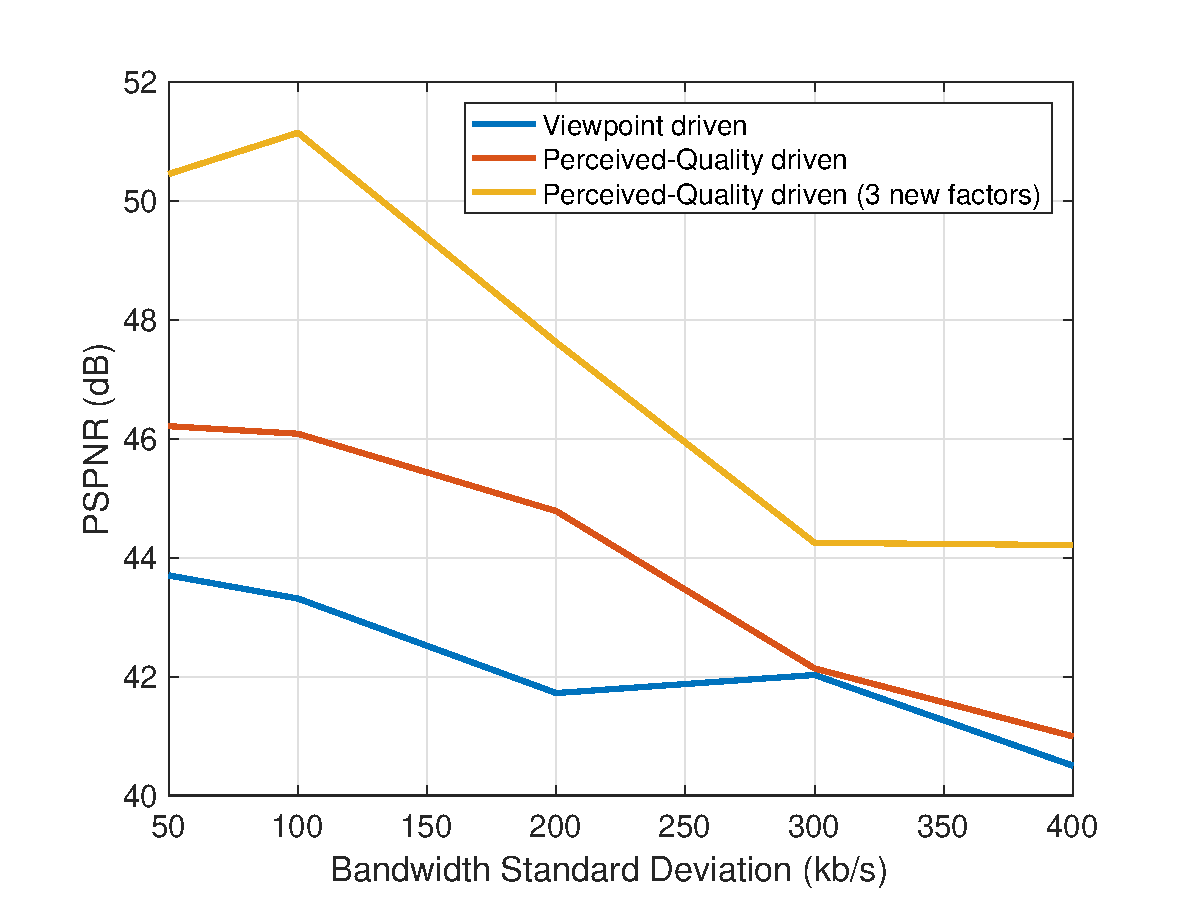
\includegraphics[width=3in]{images/throughput-PSPNR.eps}
  \caption{PSPNR of 4 methods: Viewpoint-driven, PQVRS-, PQVRS, theoretical performance.}
  \label{practical_imp}
  \end{figure}
  
    \begin{figure}
  \centering
  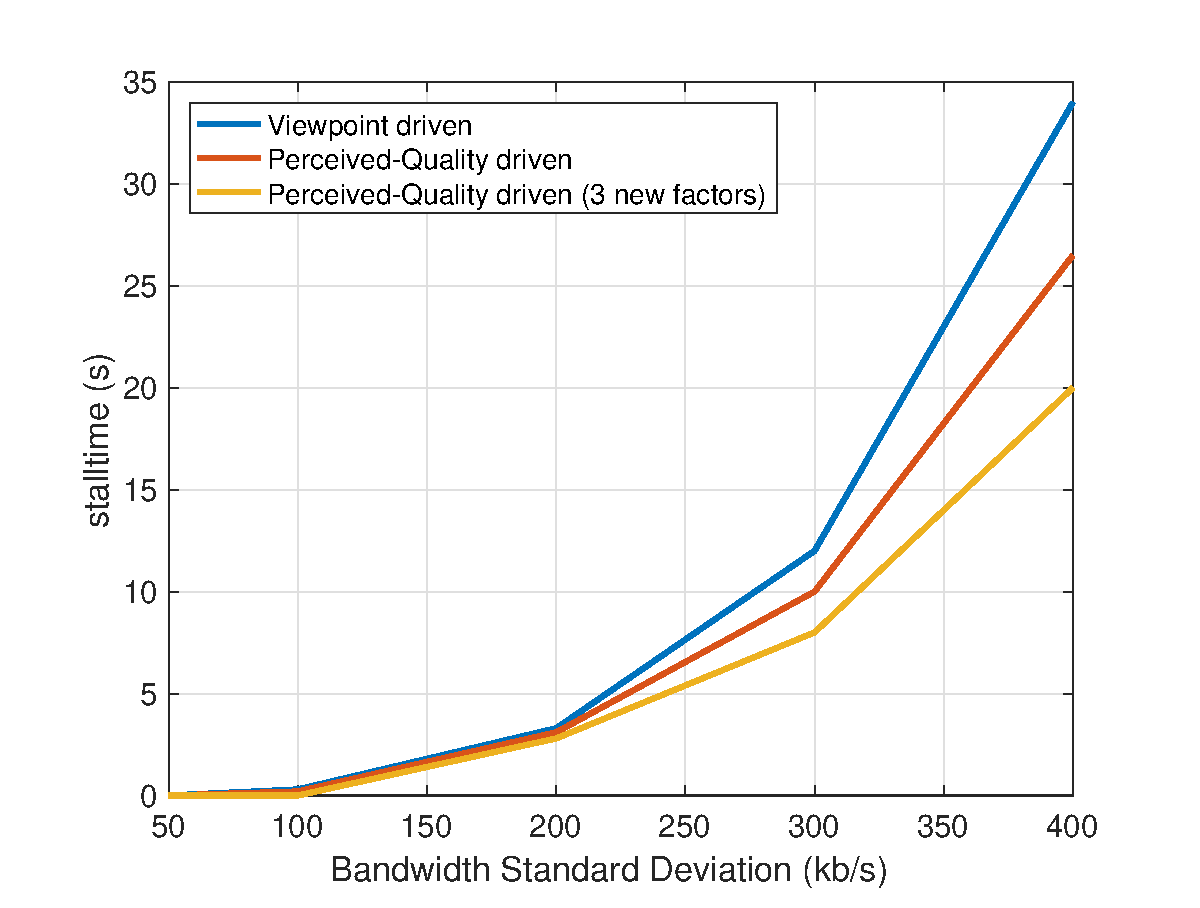
\includegraphics[width=3in]{images/throughput-stalltime.eps}
  \caption{Stalling tradeoff of 4 methods: Viewpoint-driven, PQVRS-, PQVRS, theoretical performance.}
  \label{practical_imp}
  \end{figure}

\textbf{Key observations:}

\subsection{Real-world user rating}

Based on our real-world VR streaming system, we compare above methods by real-world user rating. 

X subjects participated in the experiments. For each subject, we shown him (her) a same VR video which is streaming by Viewpoint-driven, PQVRS- and PQVRS in the same network condition. The order of display by 3 methods is random. After 3 displays, the object needs to give a rating of perceived quality for them. The rules of rating is shown in Fig. \ref{rating_rules}.

Rating rules is shown in Fig. \ref{rating_rules}. 

    \begin{figure}
  \centering
  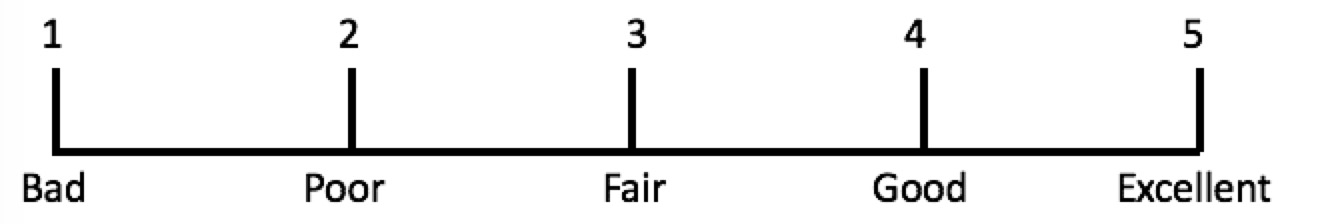
\includegraphics[width=3in]{images/rating.jpg}
  \caption{User rating rules.}
  \label{rating_rules}
  \end{figure}

Fig. \ref{rating_res} presents the result of user rating.

    \begin{figure}
  \centering
  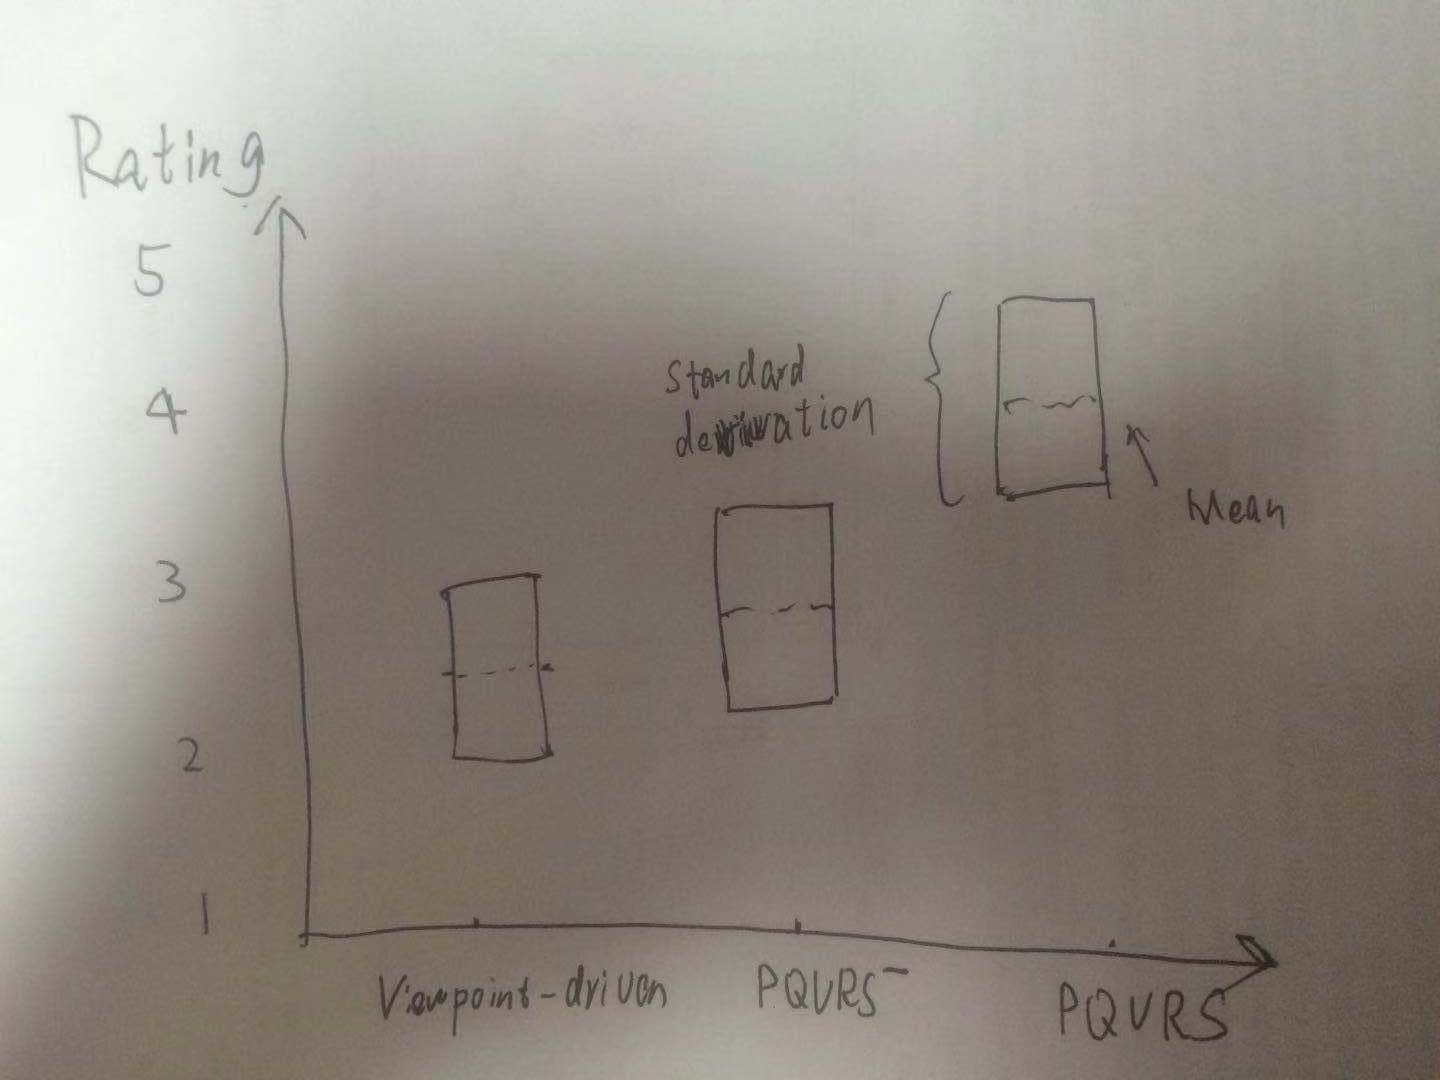
\includegraphics[width=3in]{images/rating_res.jpeg}
  \caption{User rating results.}
  \label{rating_res}
  \end{figure}

\textbf{Key observations:}

\subsection{Analysis of PQVRS improvement}

In order to clarify in which situation our proposed PQVRS has substantial improvement and in which situation it has marginal improvement, we classify our video segments according to their video types and video size.

Video types includes sports, nature, indoor, talkshow, ...

Video size is defined by the bitrate of original video. A large-size video indicates the video includes complicated or dramatically-changing content. A small-size video indicates the video includes simple and static content.

Fig. X shows the result.

    \begin{figure}
  \centering
  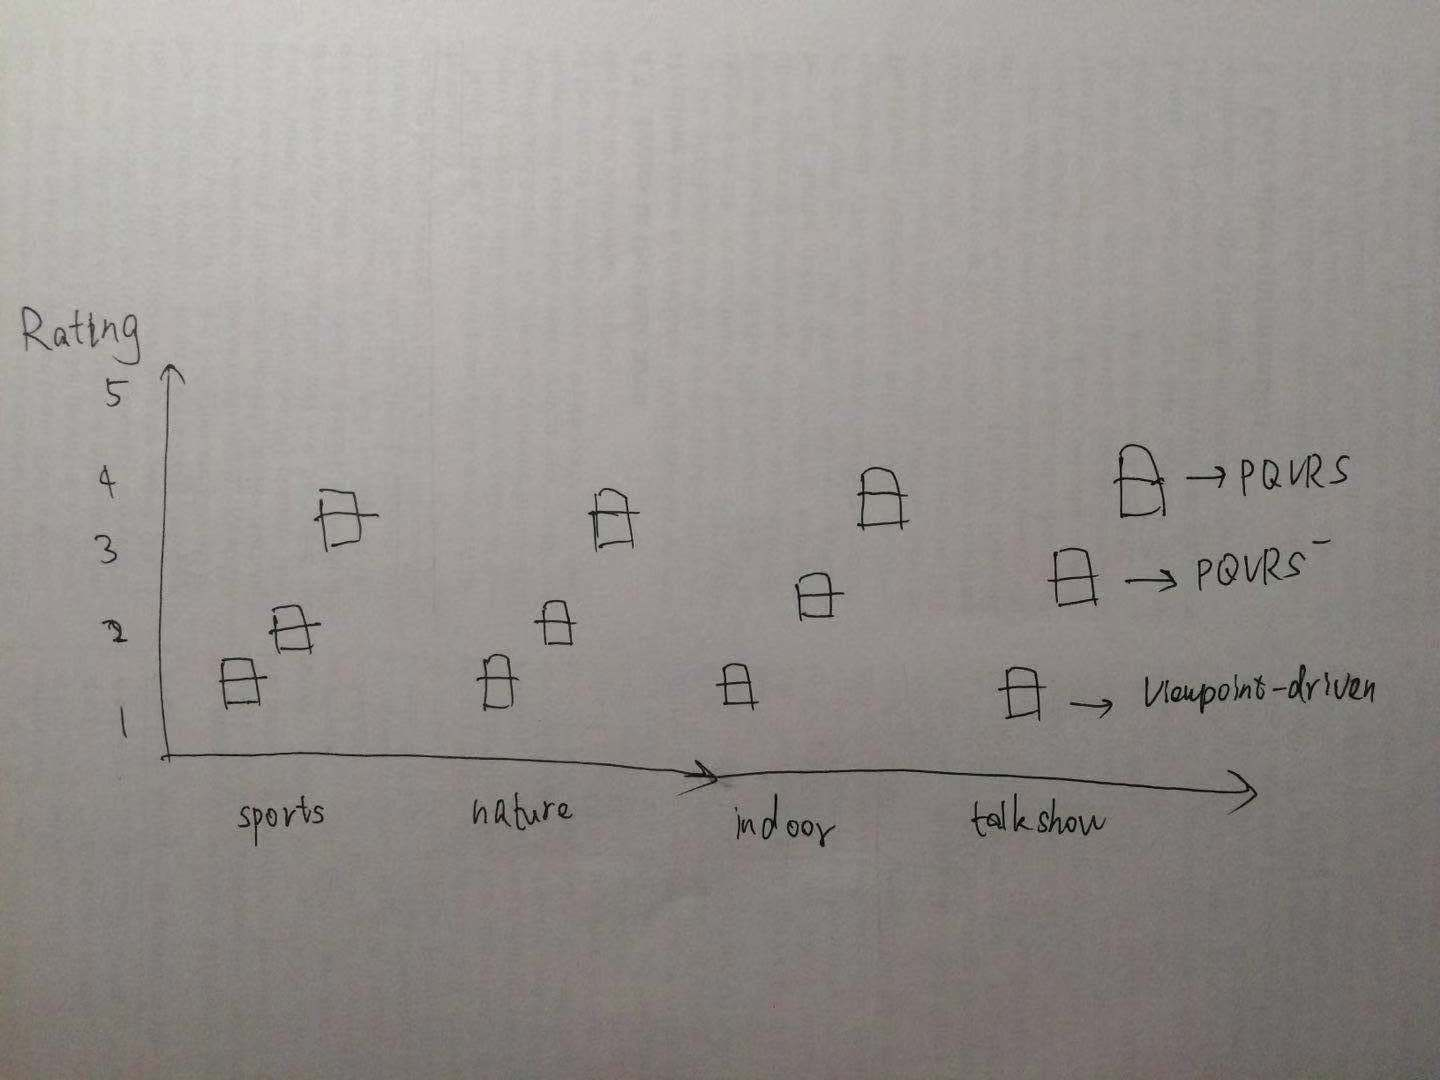
\includegraphics[width=3in]{images/rating_type.jpeg}
  \caption{User rating results for different types of videos.}
  \label{rating_res}
  \end{figure}
  
      \begin{figure}
  \centering
  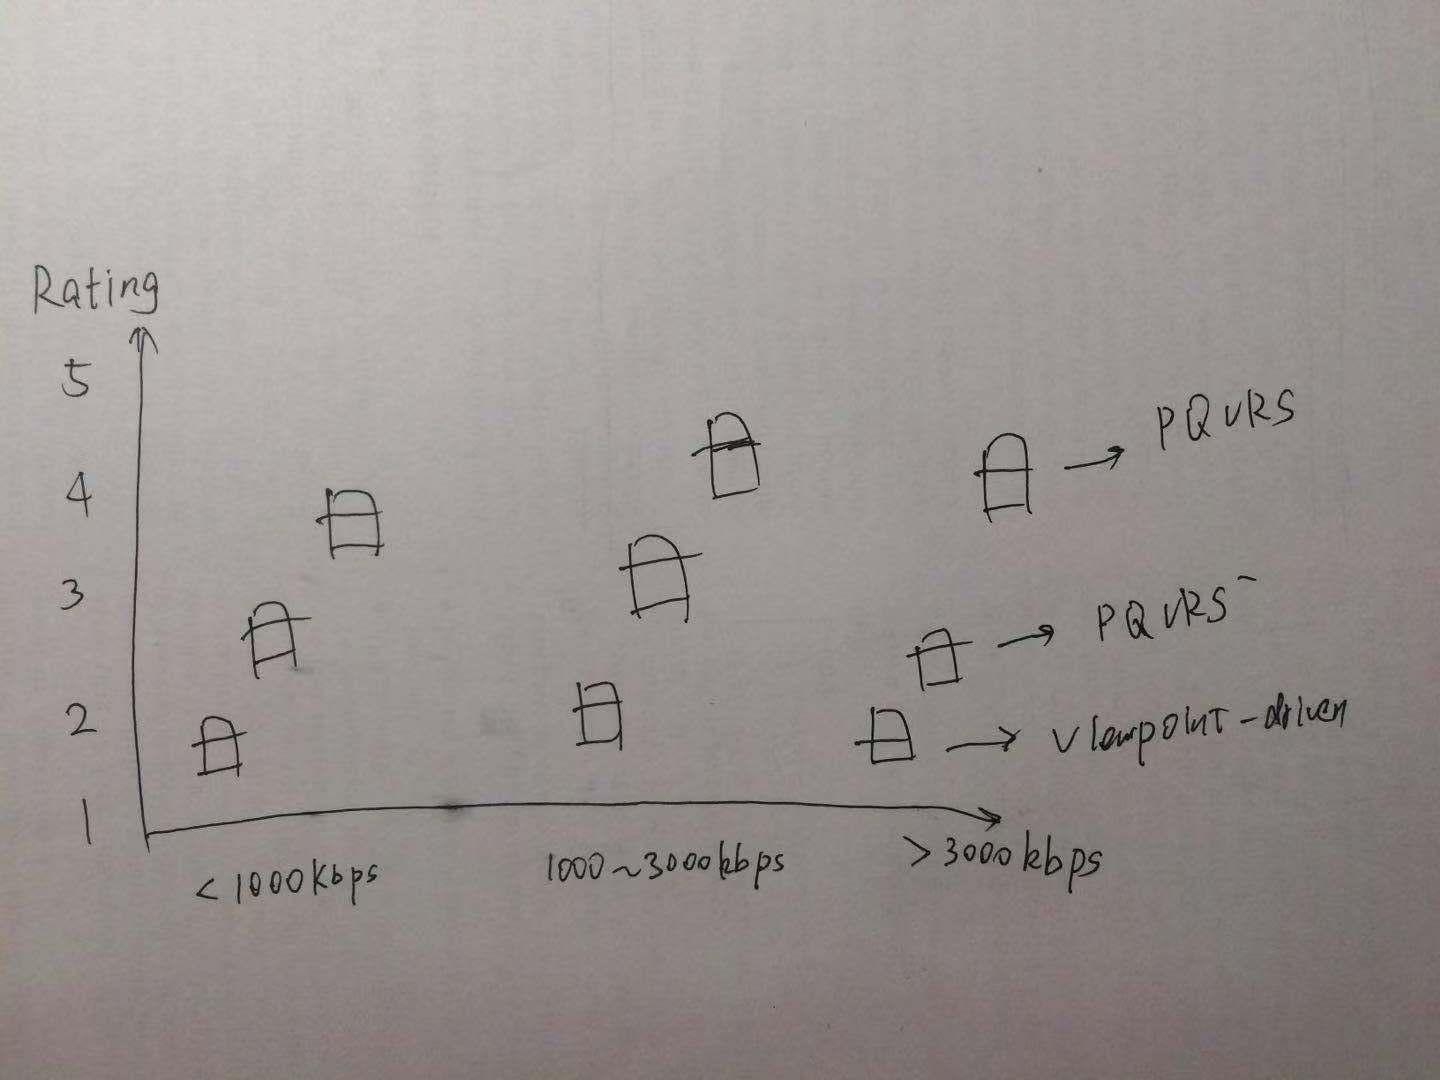
\includegraphics[width=3in]{images/rating_bitrate.jpeg}
  \caption{User rating results for videos with different original bitrate.}
  \label{rating_res}
  \end{figure}
  